\documentclass{report}
\usepackage[english]{babel}
\usepackage[utf8]{inputenc}
\usepackage[T1]{fontenc}
\usepackage{listings}
\usepackage{titlesec}
\usepackage{color}
\usepackage{graphicx}
\usepackage{geometry}
\geometry{hmargin=2.5cm,vmargin=3.5cm}

\titleformat{\chapter}[display]
            {\normalfont\bfseries}{}{0pt}{\Huge}

\lstset{ escapeinside={(*}{*)} }

\title{\textbf{Rapport IHM PROG6}\\Pingouin}

\author{Castel Antonin \and Reboul Paul \and Soret Louka \and Sorin Gaëtan \and Vandendorpe Thomas \and Eymond Laritaz Cyprien}
\begin{document}

\maketitle{}
\tableofcontents
\part*{DOSSIER}

\chapter{Introduction}
bla bla bla
\chapter{Menu}
.

\section{Scenarii}
Dans le cadre de la conception de notre interface graphique, nous avons imaginé les scenarii suivants:

\begin{itemize}
\item Scenario 1
\item Scenario 2
\item Scenario 3
\item Scenario 4
\end{itemize}

(Consulter en annexes)

 
 
 %ajouter un scenario concernant la sauvegarde et le chargement des parties
 
 \subsection{ Conclusion des scenarii }
 \begin{itemize}
  \item Nous ciblons toute personne qui souhaite passer un peu de temps sur un jeu qui pourra lui offrir un défi adapté à son profil.
  \item Une connaissance sommaire des interfaces de logiciels est suffisante pour accéder au jeu dans ses règles les plus classiques. 
  \item Quelques habitudes sont un plus pour entrer plus en fond dans le jeu et avoir une expérience plus personnalisée.
  \item Savoir lire convenablement le français permet à l'utilisateur de jouer même s'il ne connaît pas les règles.
 \end{itemize}
 
 \section{ Contraintes d'ergonomie }
 
 Afin de rendre le jeu accessible aux protagonistes, nous avons conçu un menu en deux panneaux, plus un panneau de configuration pour les joueurs plus expérimentés.
 
 \paragraph{}
 Depuis chaque menu, il est possible de revenir au menu précédent ou d'accéder à un des autres menus. Un clic depuis le menu de démarrage du jeu sur le bouton "NOUVELLE PARTIE" permet d'accéder au menu de nouvelle partie où un clic sur le bouton "Config." emmène sur le panneau de configuration de la partie. D'ici, un clic sur le bouton "Retour" ramène au menu précédent, et de la même manière sur le menu de nouvelle partie, un clic sur le bouton "retour" ramène l'utilisateur sur le menu de démarrage du jeu.

%pour les espaces:
%\hspace{0.5cm}
%\vspace{0.7cm}

\chapter{Scene de jeu}
La scène de jeu se décompose en 4 parties principales: la plateau, les scores, la panneau d'informations, les paramètres/options.

\begin{center}
  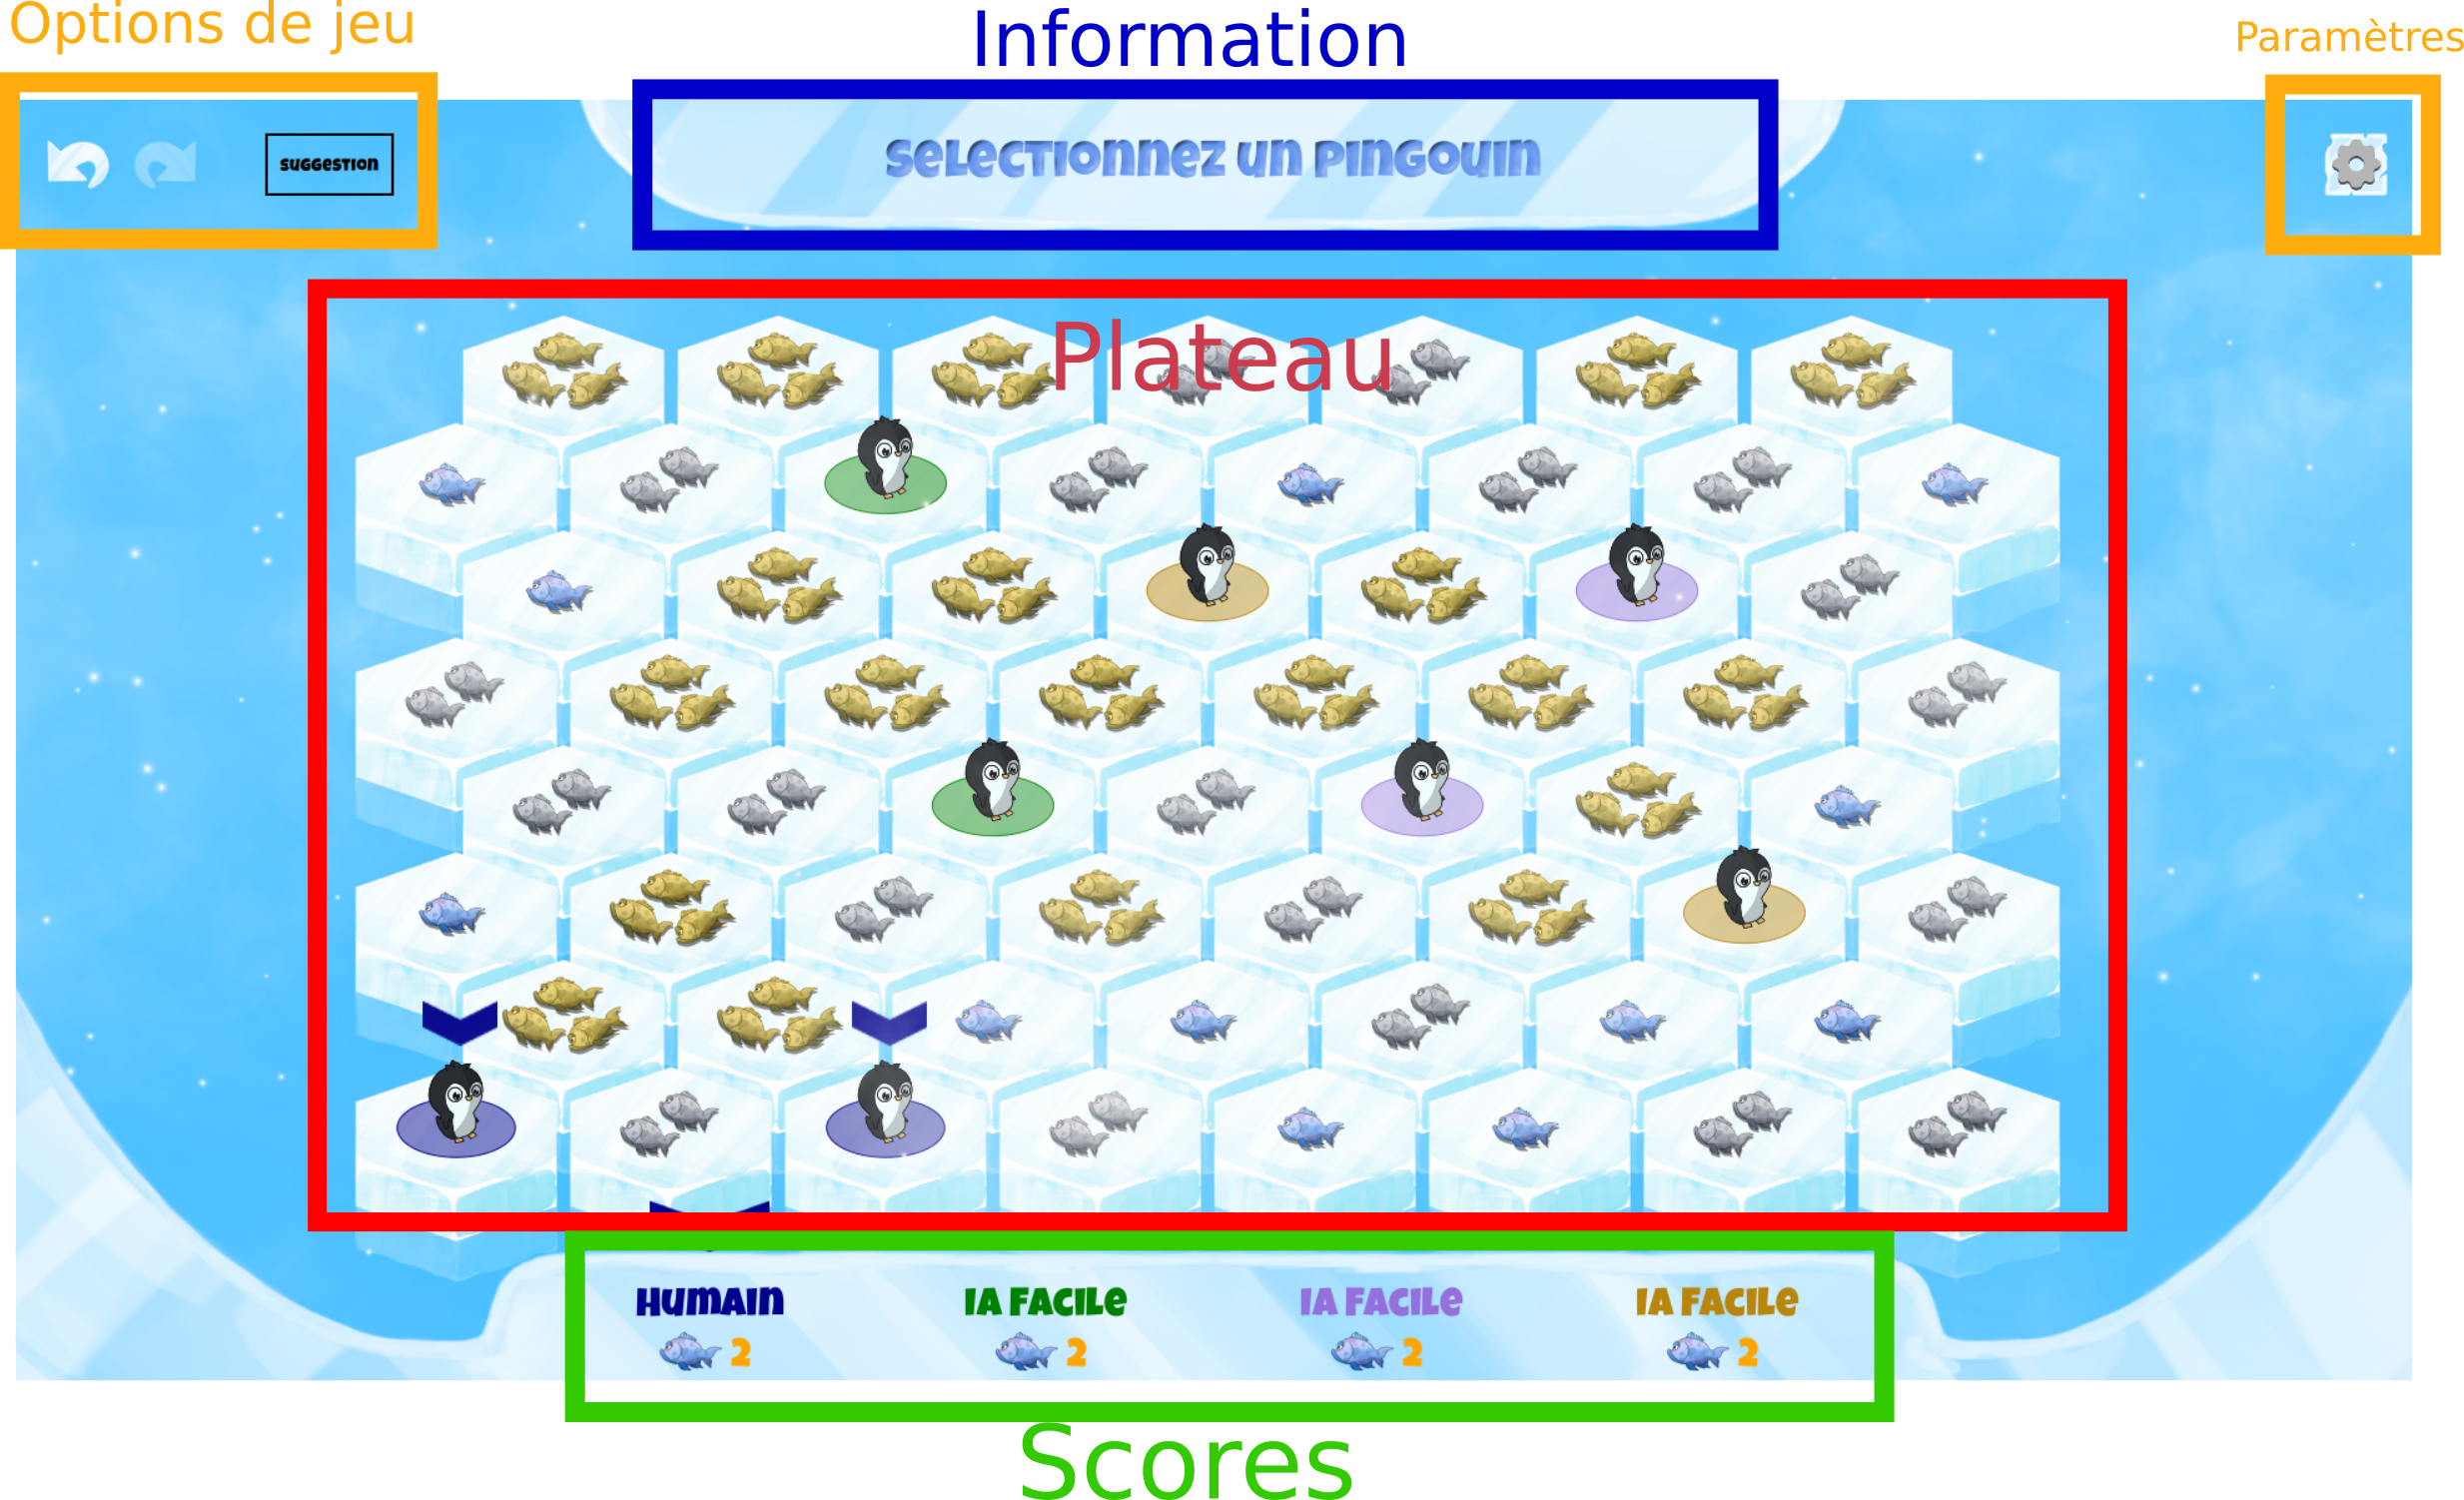
\includegraphics[width=10cm]{image/plateauIHM.png}
  \\
  Scene de jeu
\end{center}

\section{Plateau}
Le plateau est évidemment l'élément pincipal, c'est pourquoi c'est l'élément le plus grand et qu'il est centré. Cependant beaucoup d'intéractions sont possible avec ce plateau. Suite aux tests IHM,
nous avons constaté que les joueurs, lors de la première utilisation du jeu, comprennent mieux les éléments intéractifs si ces derniers sont dynamiques (clignotement, mouvement, ...). Voici comment nous avons mis en évidence les actions possibles au différentes phases du jeu.

\begin{itemize}
\item Poser un pingouin: mise en évidence des cases à un poisson lors de la phase de pose des pingouins. La couleur de la case est de la couleur du joueur courant et clignote pour signaler un objet avec lequel on peut interragir.

  \begin{center}
    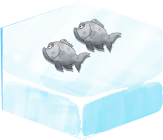
\includegraphics[width=1.5cm]{image/bloc_simple.png}    
    \hspace{1cm}
    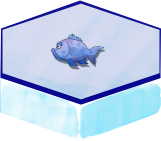
\includegraphics[width=1.5cm]{image/bloc_mev.png}
    \\
    bloc non cliquable \hspace{0.5cm} bloc cliquable
  \end{center}

\item Selectionner un pingouin: les pingouins sont tous identifiés par des ronds de la couleur de son joueur en dessous de lui. Nous avons ensuite rajouté une flèche sur les pingouins déplaçable du joueur courant. Ces flèches bougent indiquant qu'on peut intéragir avec le pingouin.
  \begin{center}
    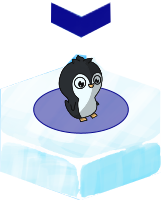
\includegraphics[width=1.5cm]{image/bloc_pingouin.png}    
  \end{center}

\item Sélectionner destinnation: le pingouin séléctionné est mis en valeur, et les cases prennent la même forme que pour la pose des pingouins.
  \begin{center}
    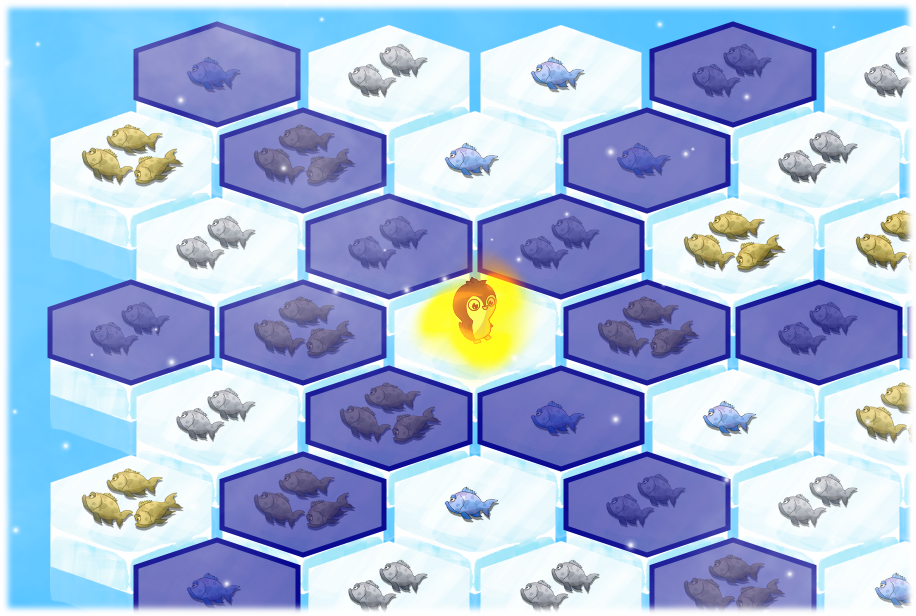
\includegraphics[width=4cm]{image/case_select_dest.png}    
  \end{center}

\item Déplacement des pingouins: lorsqu'on joue contre l'IA, il est important de montrer au joueur l'action qu'est en train de faire l'IA. Nous avons optez pour une animation lors du déplacement, les contraintes étaient d'avoir une animation visible, mais aussi rapide car si le jeu devient trop lent, il devient ennuyeux pour l'utilisateur. Ainsi lorsque le pingouin de l'IA s'apprète à bouger, il s'enflamme, puis se téléporte à sa case destinnation en laissant une trainée de flammes derrière lui.
  \begin{center}
    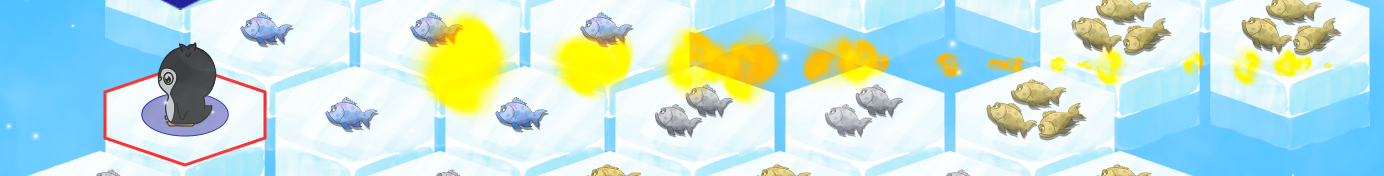
\includegraphics[width=8cm]{image/pingouin_deplacement.png}    
  \end{center}
  Nous avons géré le delai de l'animation en fonction des retours utilisateurs, lors des tests IHM, nous avons testé plusieurs delais et pris celui qui convenait le plus de joueurs.
\end{itemize}

\section{Panneau des scores}
Le joueurs doit connaître plusieurs informationd concernant l'état courant du jeu. Le panneau des scores en bas de la scène regroupe le nom des joueurs, leurs scores (nombre de poissons mangés), ainsi que le nombre de pingouins qu'il reste à poser (lors de la phase de pose des pingouins). On se sert également de ce panneau pour indiquer le joueur courant à l'aide d'une flêche, bien que nous nous sommes rendus compte que les utilisateurs regardent plutôt les informations du plateau (flèche au dessus des pingouins) pour savoir qui doit jouer.
  \begin{center}
    
\includegraphics[width=8cm]{image/tableau_scores.png}    
  \end{center}

\section{Panneau d'information}
Nous avons souhaité qu'un joueur puisse constamment savoir qu'elle action il doit faire (même s'il ne connait pas les règles du jeu). C'est pourquoi, en plus d'avoir des éléments dynamiques sur le plateau l'insitant à intéragir, il existe aussi un panneau informant de ce que doit faire le joueur: ``Poser un pingouin'', ``Selectionner un pingouin'', ``Selectionner une destinnation'', ``Attendre son tour''. Au fil des tests utilisateurs, nous avons dû augmenter la taille du panneau afin de le mettre plus en évidence. En effet nous avons pu constater que tous les utilisateurs n'ont pas le réflex de lire alors que ce panneau peut être important lors des premières parties d'un joueur.

\section{Paramètres et options}
Nous avons choisi de placer les boutons non essentiels au jeu au même endroit qu'on peut les trouver dans d'autre logiciel, afin de ne pas trop changer les habitudes des utilisateurs. Nous avons donc le undo/redo en haut à gauche et les paramètres en haut à droite. Voici quelques remarques interessantes concernant ces options:

\begin{itemize}
\item Boutons grisés: Certains des boutons peuvent parfois ne pas être activables, ils sont alors grisés. C'est les cas des boutons undo/redo lorqu'on est à une extrémité de l'historique par exemple.

\item Distance par rapport au plateau: On nous a alerté de la distance au plateau des boutons undo/redo lors des audits IHM pour minimiser le déplacement de souris. Nous n'avons pas souhaité les rapprocher, bien que nous ayons un peu augmenté la taille du plateau depuis. Nous justifions ce choix par:
  \begin {enumerate}
  \item cela ne semblait pas poser de problèmes lors des tests utilisateurs
  \item nous pensons que le nombre de fois où un joueur utilise undo/redo dans une partie n'est pas assez important pour justifier une place trop prèt du plateau
  \item trop prêt du plateau, ces boutons peuvent devenir génants (lors d'un miss clic par exemple)
  \end{enumerate}

\item Bouton paramètre: lorsqu'on clique sur ce bouton, un petit menu apparaît en haut à droite de la fenêtre. Ce petit menu apparaîssait autrefois au centre, mais nous l'avons déplacé pour minimiser le déplacement de souris.
  \\
  \\
\begin{minipage}{0.3\linewidth}
 % \begin{center}
    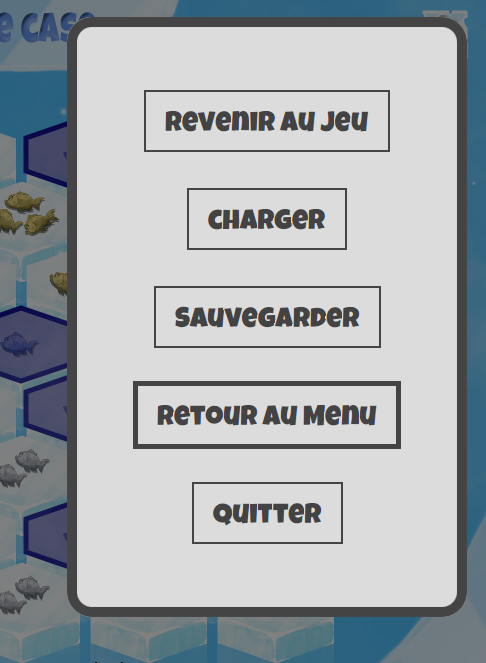
\includegraphics[width=4cm]{image/parametres.png}    
    % \end{center}
\end{minipage}\hfill
\begin{minipage}{0.7\linewidth}
    Les boutons ``sauvegarder''/''charger'' ouvrent une fenêtre de choix de fichier. Le bouton ``quitter'' ouvre une fenêtre de confirmation pour éviter que la fenêtre ne se ferme trop brutalement (remarques issues des tests utilisateurs).
  \end{minipage}
\end{itemize}

\section{Retour tests utilisateurs}
(VOIR ANNEXE pour une fiche d'exemple d'évaluation d'utilisateur)
On peut catégoriser les retours des tests utilisateurs en 2 parties.
\begin{itemize}
\item Les retours attendus, qui correspondent aux questions/actions qu'on voulait tester et qui étaient préalablement écrites dans les feuilles utilisées pour évaluer l'utilisateur.
\item Les remarques et comportements des  utilisateurs.
\end{itemize}

\subsection{Les retour attendus}
Nous avons demandé au utilisateurs d'effectuer certaines actions, et nous avons coché ``echec'', ``facile'', ``moyen'' ou  ``difficile'' en fonction de la réussite de l'utilisateur. Nous avons ensuite pu déterminer où concentrer nos efforts sur l'application.

Nous avons construit un graphique (fourni en annexe), en attribuant une valeur (entre 0 et 3) à la réussite de l'utilisateur. Sur ce graphique, nous pouvons voir que nous avons dû retravailler l'indication du joueur courant et des scores, ainsi que la configuration d'une partie.

\subsection{Les remarques et comportements des utilisateurs}
Nous avons aussi appris beaucoup en écoutant et en observant les utilisateurs, sur des choses auxquelles nous n'avions pas pensées ou qui ne s'adaptaient pas au questionnaire précédent:
\begin{itemize}
\item Afficher le nombre de pingouins restant à la phase de pose
\item Gérer les delais entre chaque tour
\item Certaines couleurs de joueurs étaient peu visibles
\item Ne pas quitter la partie trop brutalement lorsqu'on clique sur ``quitter''
\item Le temps pour trouver les éléments cliquable est diminué si ces éléments sont mis en évidence dynamiquement (clignotement, fleche en mouvement, changement d'affichage lors du passage de la souris)
\end{itemize}


\part*{ANNEXES}

\begin{tabular}{|c|l|}
 \hline
 \multicolumn{2}{|c|}{Scenario 1}\\
 \hline
 Protagoniste(s) & Un enfant E, en âge de lire et ayant déjà utilisé une interface logicielle \\
 \hline
 Contexte(s) & \parbox{13cm} {\begin{itemize}
 	\item E est laissé seul devant un ordinateur avec le jeu des pingouins lancé en plein écran. Il ne connaît pas les règles du jeu
\end{itemize} }\\
 \hline
 Scenario & \parbox{13cm}{ E souhaite faire une partie. Il n'a aucune idée de l'existence d'une fonction pour modifier la configuration du jeu, ni ne connaît les règles. Sa connaissance de la langue française lui permet d'inférer que le bouton "NOUVELLE PARTIE" en évidence le rapproche de son objectif: démarrer une partie. \\
 Il arrive sur un panneau où il trouve trois boutons, "Config." en petit, "JOUER" en plus gros, et "Retour" en petit à nouveau. Il clique naturellement sur le bouton "JOUER", et la partie avec les règles de bases se lance, à savoir 4 joueurs, avec le joueur humain qui commence, avec chacun deux pingouins. Il ne connaît pas les règles et a la présence d'esprit de regarder les éléments d'interface à sa disposition. Il tombe sur un court texte lui décrivant les actions qu'il peut faire à tout moment. En suivant les indications, il parvient à terminer sa première partie.} \\
 \hline
 \end{tabular}

\vspace{0.4cm} 
 
  \begin{tabular}{|c|l|}
  \hline
 \multicolumn{2}{|c|}{Scenario 2}\\
 \hline
 Protagoniste(s) & Une personne P plus habituée aux jeux-vidéo ou aux jeux de société \\
 \hline
 Contexte(s) & \parbox{13cm} {\begin{itemize}
 	\item P lance avec envie le jeu des pingouins dans l'optique de chercher un défi à sa hauteur
\end{itemize} }\\
 \hline
 Scenario & \parbox{13cm}{ P, de part son expérience avec les logiciels et jeux vidéos, analyse sans mal la logique de l'interface des menus après plusieurs parties, constate qu'il arrive avec une facilité déconcertante à gagner l'intégralité des parties qu'il mène. Voulant passer à la vitesse supérieure, il décide de cliquer sur les flèches près de l'image de la banquise afin de démarrer en mode "ENFER", tel que marqué dans le titre. Il joue alors contre des IA Difficiles.} \\
 \hline
 \end{tabular}
 
\vspace{0.4cm} 
 
 \begin{tabular}{|c|l|}
 \hline
 \multicolumn{2}{|c|}{Scenario 3}\\
 \hline
 Protagoniste(s) & Un habitué H qui utilise le jeu depuis un moment déjà. \\
 \hline
 Contexte(s) & \parbox{13cm} {\begin{itemize}
 	\item H utilise le jeu depuis quelques parties et pense avoir fait le tour.
 	\item H peut être P du scénario précédent, après avoir gagné ou perdu un nombre suffisamment grand pour vouloir essayer de nouvelles expériences
\end{itemize} }\\
 \hline
 Scenario & \parbox{13cm}{  Au bout d'un certain nombre de parties, H clique sur le bouton "config" afin d'explorer un monde d'options insoupçonné qui n'attendait que d'être découvert. Il découvre alors qu'il peut non seulement changer le nombre de joueurs, mais aussi leur difficulté et le nombre de leurs pingouins de manière individuelle. Il peut alors observer des matches composées uniquement d'IA si ça l'intéresse, ou même réduire le terrain de jeu à son minimum, ou encore explorer un champs de parties où le nombre de cases à trois poissons est largement supérieur au nombre des autres cases. \\
 Si H est P du scénario précédent, il sera heureux de découvrir un mode de difficulté supérieur, à savoir par exemple un nombre réduit de pingouins pour sa part par rapport à ses adversaires. Si ce dernier, en revanche a été mis en échec par les IA difficiles en mode ENFER, il pourra au contraire adapter parfaitement la difficulté à son niveau de jeu en faisant varier le nombre de pingouins et la difficulté des joueurs associés. } \\
 \hline
 \end{tabular}

\vspace{0.4cm}

\begin{tabular}{|c|l|}
\hline
 \multicolumn{2}{|c|}{Scenario 4}\\
 \hline
 Protagoniste(s) & Deux amis A1 et A2 souhaitant s'amuser entre eux avec un jeu bon enfant \\
 \hline
 Contexte(s) & \parbox{13cm} {\begin{itemize}
 	\item A1 et A2 sont à deux sur la même machine
 	\item A1 et A2 ont éventuellement une souris branchée par personne
\end{itemize} }\\
 \hline
 Scenario & \parbox{13cm}{  A1 et A2 souhaitent jouer ensemble au jeu des pingouins. Par le même procédé que le précédent, ils peuvent configurer un duel de deux joueurs humains et jouer l'un contre l'autre. \\
 Si A1 et A2 se sont renommés dans le menu de configuration en effectuant un clic droit sur "HUMAIN", ils pourront partager leurs performances avec une capture d'écran pour montrer que l'un joue mieux que son ami. \\
 Si l'un des amis joue mieux que l'autre, ils peuvent, par le même procédé que celui décrit dans le scénario précédent, permettre à l'un de poser plus de pingouins que l'autre en début de partie pour ainsi rééquilibrer leur rapport de force et ainsi rester amis.} \\
 \hline
\end{tabular}

\newpage
\begin{center}
  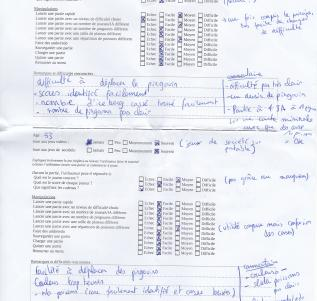
\includegraphics[width=12cm]{image/testut.jpg}
  \\
  Exemple d'une fiche utilisée pour évaluer un utilisateur
  \\
  \vspace{1cm}
  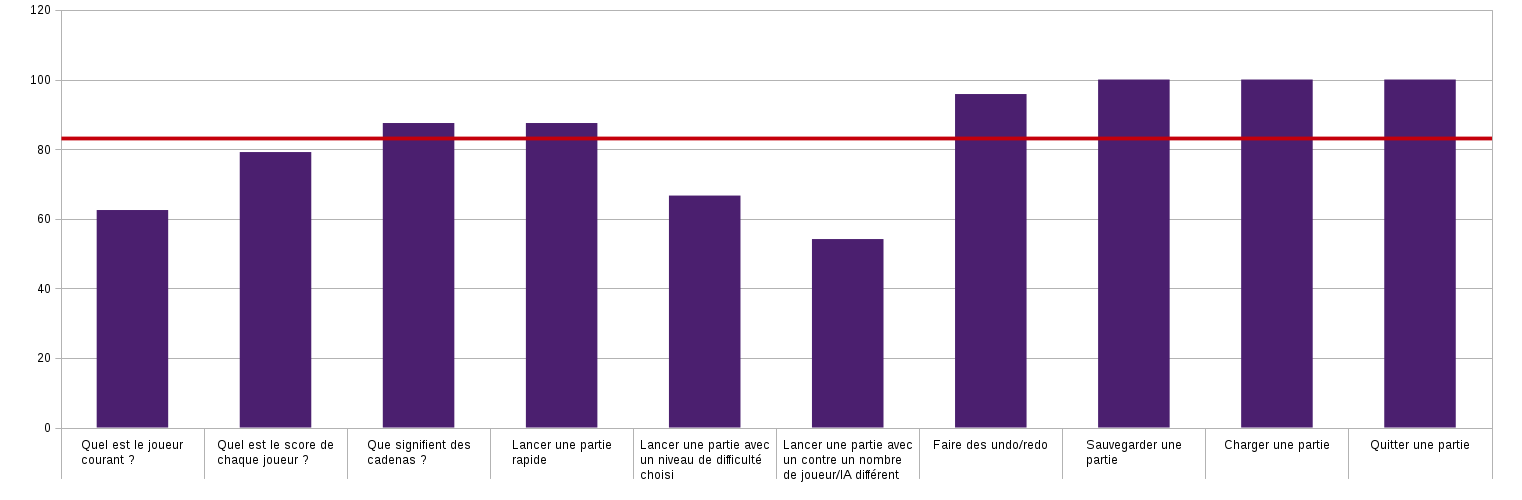
\includegraphics[width=15cm]{image/graphIHM.png}
  \\
  Pourcentage de réussite de tous les utilisateurs sur les actions demandées. (La réussite est une valeur entre 0 à 3 pour ``echec'',''difficile'',''moyen'',''facile'')
\end{center}

\newpage
\begin{center}
  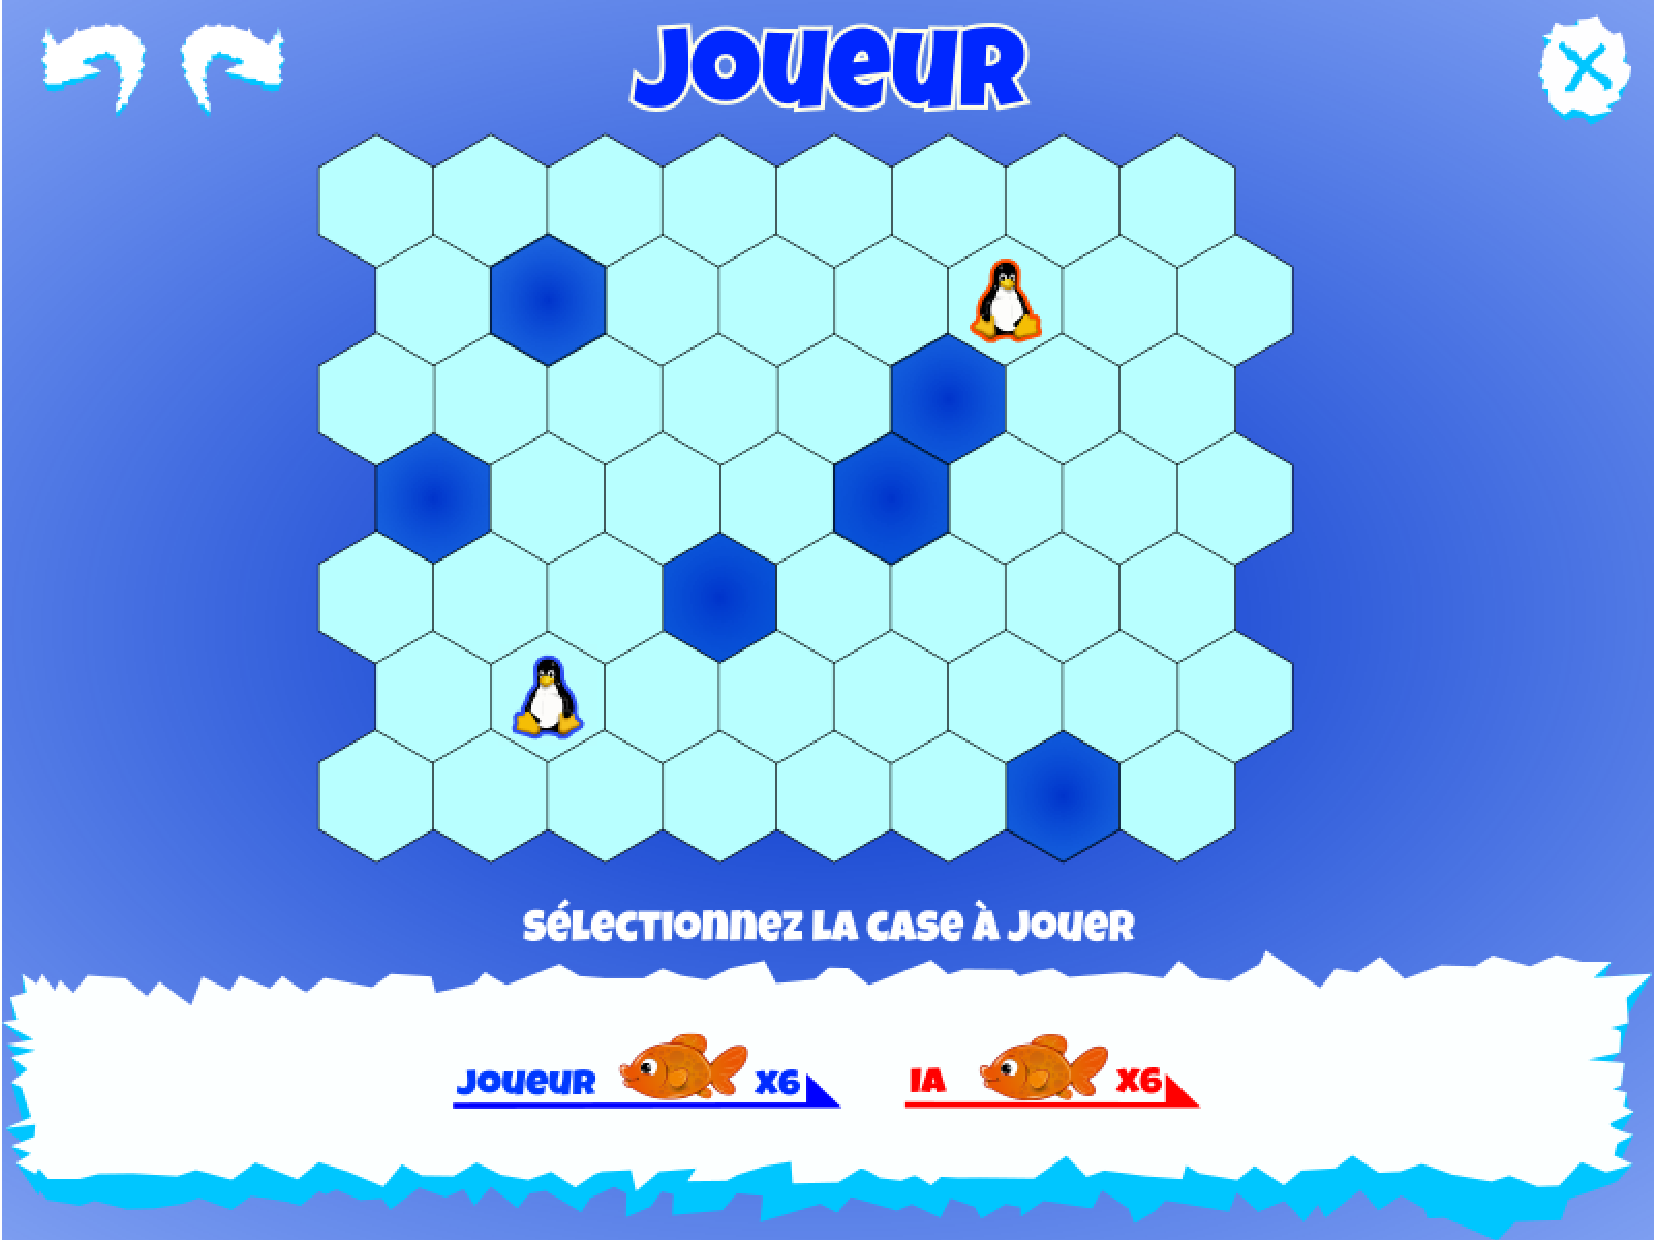
\includegraphics[width=7cm]{image/ancienPlateau.pdf}
  \\
  Maquette
  \\
  \vspace{1cm}
  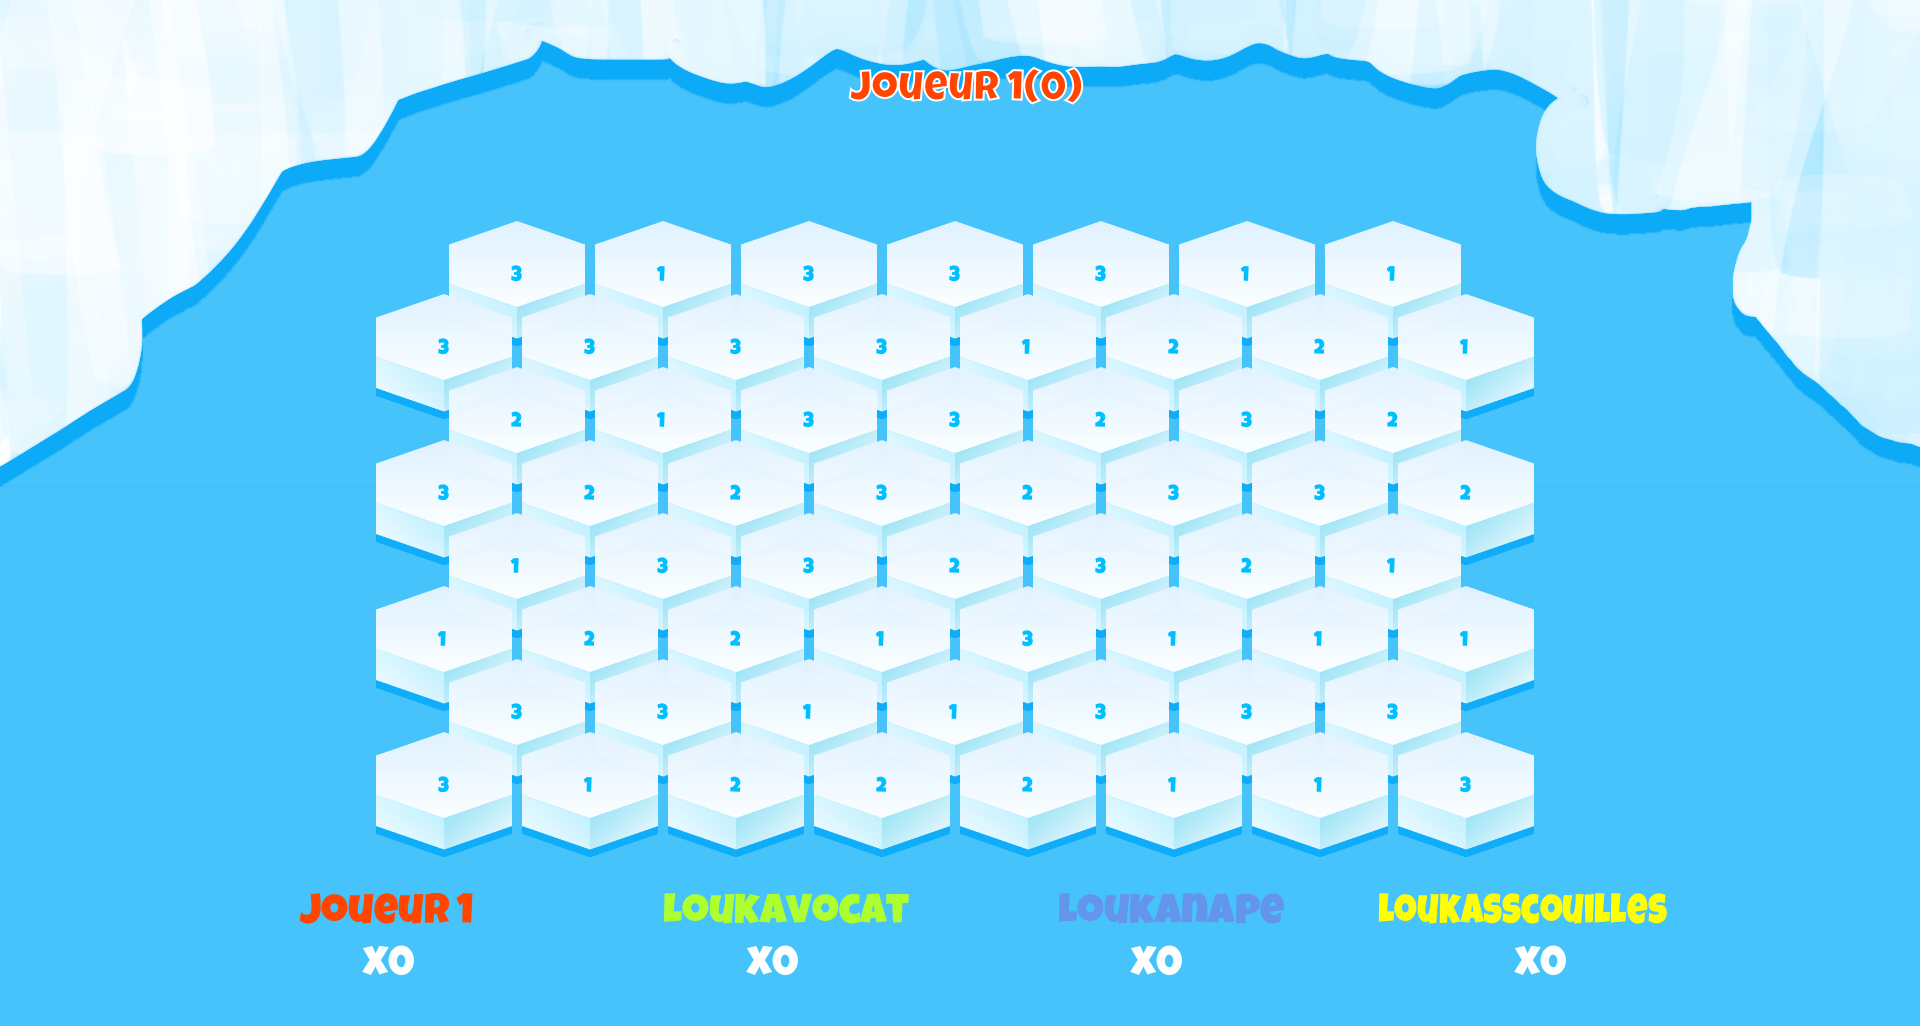
\includegraphics[width=7cm]{image/version2.png}
  \\
  Première version
  \\
   \vspace{1cm}
  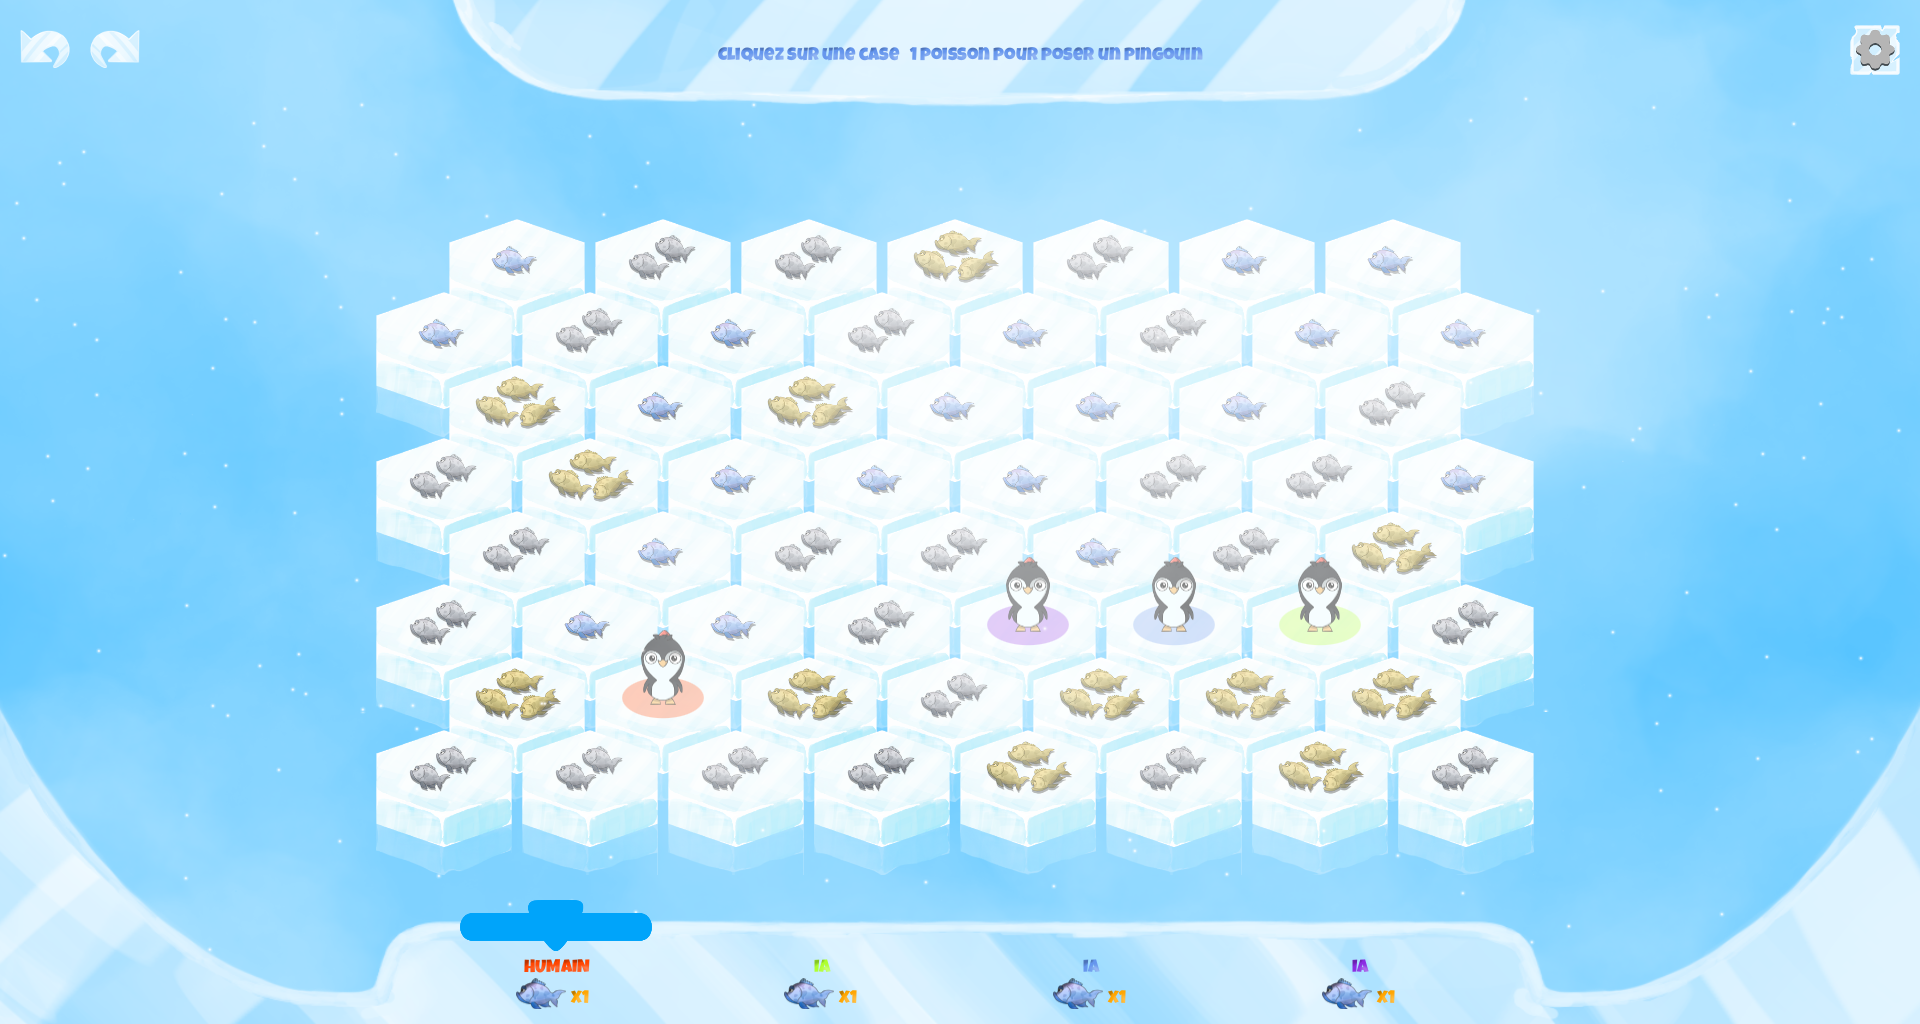
\includegraphics[width=7cm]{image/version3.png}
  \\
  Seconde version
  \\
   \vspace{1cm}
  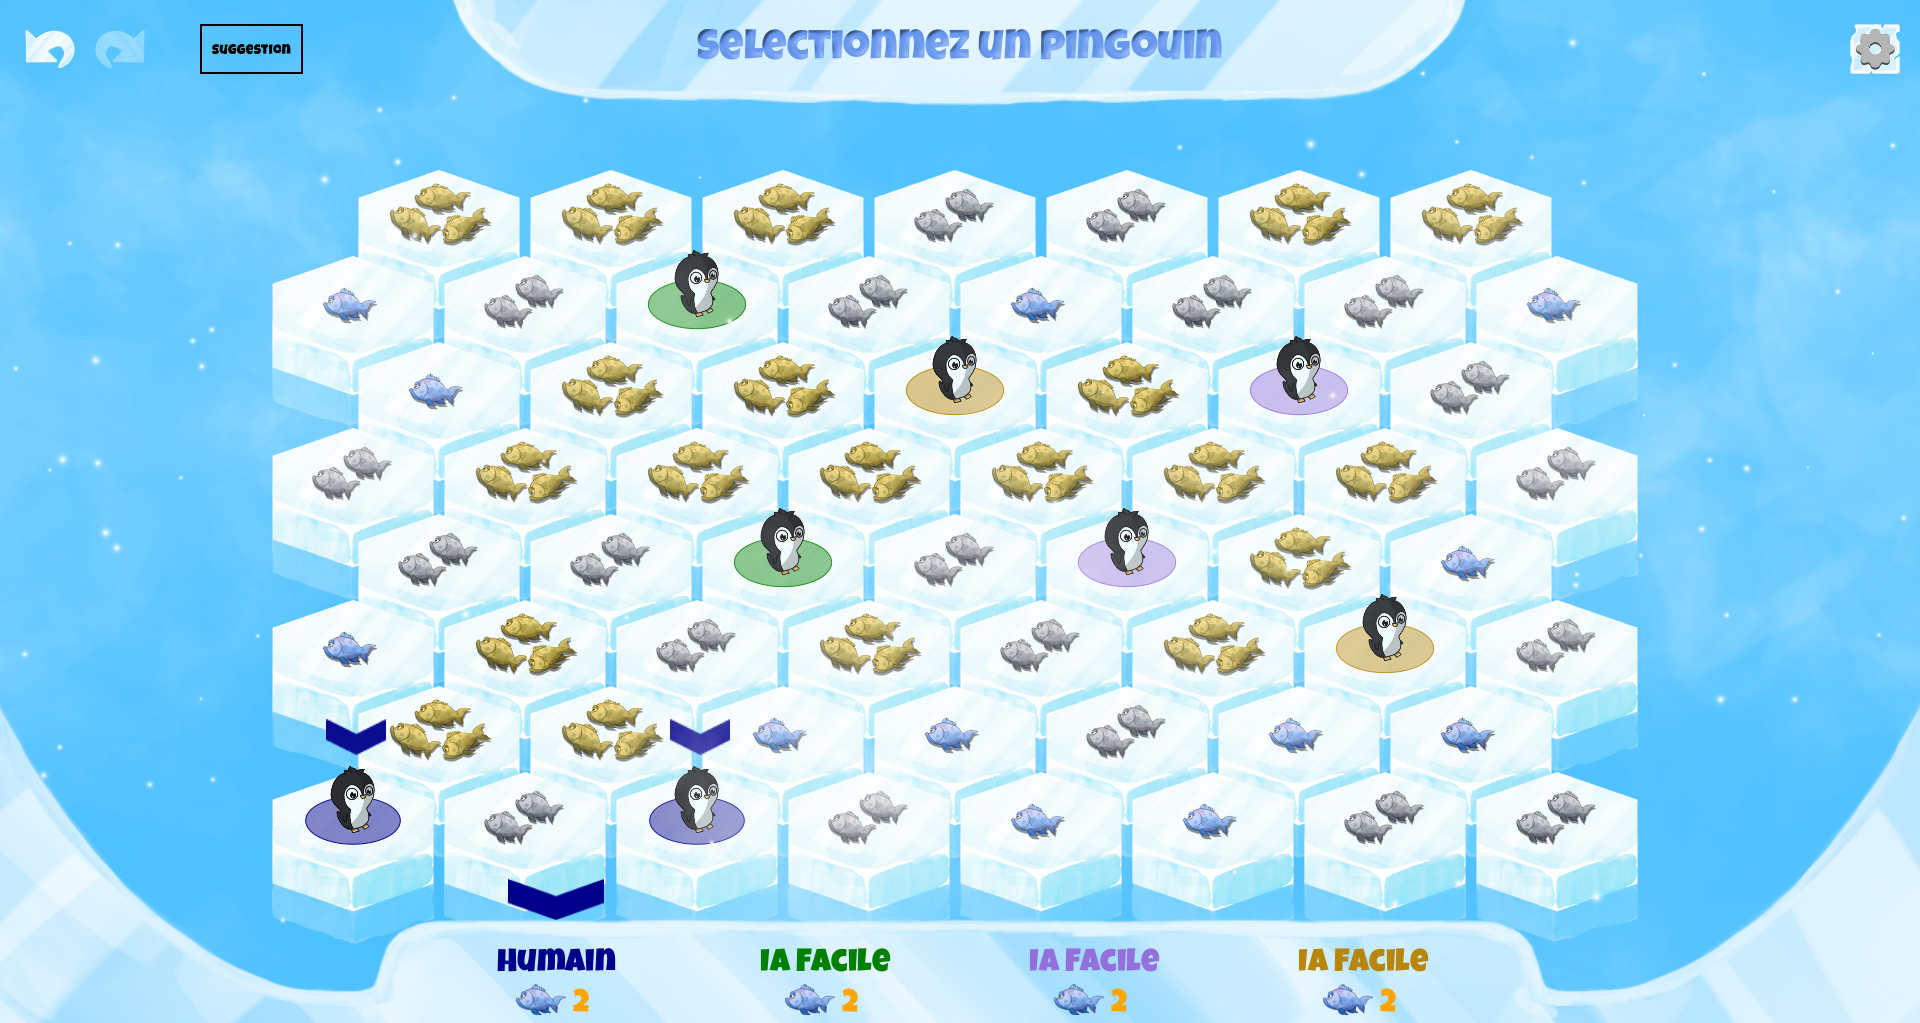
\includegraphics[width=6cm]{image/version4.png}
  \\
  Troisième version
  \\
\end{center}

\end{document}
